\documentclass[mathserif, handout]{beamer}
% ======================================================================
% General LaTeX Setup for Beamer (Reusable Preamble)
% Author: Chandra Gummaluru
% ======================================================================

\documentclass[mathserif, handout]{beamer}
\setbeamertemplate{frametitle}{}

% ------------------------------------------------------------
% basic packages
% ------------------------------------------------------------
\usepackage{url}
\usepackage{ifthen}
\usepackage{enumerate}
\usepackage[font=small]{caption}
\usepackage{subcaption}
\usepackage{moresize}
\usepackage[outline]{contour}
\usepackage{transparent}
\usepackage{worldflags}
\usepackage{bm}
\usepackage{graphbox}
\usepackage{mathtools}
\usepackage{multirow}
\usepackage{fontawesome5}
\usepackage{pifont}
\usepackage{array}
\usepackage{comment}

% ------------------------------------------------------------
% math
% ------------------------------------------------------------
\DeclarePairedDelimiter{\floor}{\lfloor}{\rfloor}
\DeclarePairedDelimiter{\ceil}{\lceil}{\rceil}

% ------------------------------------------------------------
% colors
% ------------------------------------------------------------
\definecolor{hl}{RGB}{248,196,69}
\definecolor{myred}{HTML}{ED5565}
\definecolor{myorange}{HTML}{FC6E51}
\definecolor{myyellow}{HTML}{FFCE54}
\definecolor{mycyan}{HTML}{4FC1E9}
\definecolor{myblue}{HTML}{5D9CEC}

\newcommand{\graytext}[1]{\footnotesize\color{gray}#1\normalsize\color{black}}

% ------------------------------------------------------------
% symbols
% ------------------------------------------------------------
\newcommand{\cmark}{\ding{51}}
\newcommand{\xmark}{\ding{55}}

% ------------------------------------------------------------
% highlighting
% ------------------------------------------------------------
\newcommand{\reducedstrut}{\vrule width 0pt height .9\ht\strutbox depth .9\dp\strutbox\relax}
\newcommand{\highlight}[1]{%
  \begingroup\setlength{\fboxsep}{0pt}\colorbox{hl}{\reducedstrut$\displaystyle #1$\/}\endgroup}
\newcommand{\highlightc}[2]{%
  \begingroup\setlength{\fboxsep}{0pt}\colorbox{#1}{\reducedstrut$\displaystyle #2$\/}\endgroup}

% ------------------------------------------------------------
% environments (boxes)
% ------------------------------------------------------------
\usepackage{tcolorbox}
\tcbuselibrary{skins}

\newtcolorbox{thmbox}[1][]{colback=gray!30!white!20, colframe=black, fonttitle=\bfseries, title=#1, boxrule=0.5pt}

% 1) Bottom open (draw top + sides only)
\newtcolorbox{thmboxtop}[1][]{
    enhanced,
    frame hidden,
    colback=gray!30!white!20,
    borderline north={0.5pt}{0pt}{black}, % top
    borderline west={0.5pt}{0pt}{black},  % left
    borderline east={0.5pt}{0pt}{black}   % right
}

% 2) Top open (draw bottom + sides only)
\newtcolorbox{thmboxbot}[1][]{
    enhanced,
    frame hidden,
    colback=gray!30!white!20,
    borderline south={0.5pt}{0pt}{black}, % bottom
    borderline west={0.5pt}{0pt}{black},  % left
    borderline east={0.5pt}{0pt}{black}   % right
}

% 3) Side only (draw only left and right)
\newtcolorbox{thmboxside}[1][]{
    enhanced,
    frame hidden,
    colback=gray!30!white!20,
    borderline west={0.5pt}{0pt}{black},  % left
    borderline east={0.5pt}{0pt}{black}   % right
}

\newtcolorbox{defboxtop}[1][]{
    enhanced,
    colback=gray!30!white!20,
    frame hidden,
    overlay={
        % Draw top + sides with rounded corners
        \draw[line width=0.5pt, black, rounded corners=3mm]
            (frame.south west) -- (frame.north west) -- (frame.north east) -- (frame.south east);
    },
    #1
}

\newtcolorbox{defboxbot}[1][]{
    enhanced,
    colback=gray!30!white!20,
    frame hidden,
    overlay={
        % Draw top + sides with rounded corners
        \draw[line width=0.5pt, black, rounded corners=3mm]
            (frame.north west) -- (frame.south west) -- (frame.south east) -- (frame.north east);
    },
    #1
}

\newtcolorbox{defboxside}[1][]{
    enhanced,
    frame hidden,
    colback=gray!30!white!20,
    borderline west={0.5pt}{0pt}{black},  % left
    borderline east={0.5pt}{0pt}{black}   % right
}

\newtcolorbox{proofbox}[1][]{colback=gray!20!white!20, colframe=grey, fonttitle=\bfseries, title=#1, boxrule=0.5pt, colbacktitle=white, enhanced jigsaw, sharp corners}

% ------------------------------------------------------------
% code listings
% ------------------------------------------------------------
\usepackage{listings}
\lstdefinestyle{mypython}{
  language=Python,
  deletekeywords=[2]{open, next, from, chr, str, int},
  morekeywords=[3]{List, Graph, Tree, Dict, Set, UnionFind, Ordict, Trie, Queue},
  morekeywords=[4]{ListNode, Vertex, Edge, Path, TreeNode, DictNode, UnifNode, OrdictNode, TrieNode, QueueNode},
  morekeywords=[5]{True, False, Boolean, String, Integer, Key, Function, KeyedObject, Object, Array, Tuple, Optional, None},
  keywordstyle=\color{mycyan}\bfseries,
  keywordstyle=[3]\color{myblue}\bfseries,
keywordstyle=[4]\color{myblue}\bfseries,
keywordstyle=[5]\color{mycyan}\bfseries,
  stringstyle=\color{orange},
  commentstyle=\color{gray}\itshape,
  basicstyle=\ttfamily\footnotesize,
  numbers=left,
  numberstyle=\tiny\color{gray},
  stepnumber=1,
  numbersep=5pt,
  xleftmargin=15pt,
  frame=none,
  showstringspaces=false,
  breaklines=true,
  breakatwhitespace=true,
  tabsize=4,
  columns=flexible
}


% ------------------------------------------------------------
% algorithms
% ------------------------------------------------------------
\usepackage{algorithm}
\usepackage[endLComment=~]{algpseudocodex}
\makeatletter
\algrenewcommand\ALG@beginalgorithmic{\footnotesize}
\makeatother

% ------------------------------------------------------------
% optimization environments
% ------------------------------------------------------------
\usepackage[nocomma]{optidef}

% ------------------------------------------------------------
% pgfplots and pie charts
% ------------------------------------------------------------
\usepackage{pgfplots}
\usepackage{pgf-pie}
\pgfplotsset{compat=1.7}

% ------------------------------------------------------------
% tikz
% ------------------------------------------------------------
\usepackage{tikz}
\usetikzlibrary{
  angles, quotes, positioning, fit, backgrounds, shapes.geometric, intersections,
  calc, shapes, mindmap, decorations.text, arrows, arrows.meta,
  automata, chains, decorations.pathreplacing, calligraphy,
  decorations.markings, shapes.misc, decorations.pathmorphing
}
\tikzset{
  invisible/.style={opacity=0},
  visible on/.style={alt=#1{}{invisible}},
  alt/.code args={<#1>#2#3}{\alt<#1>{\pgfprioritysalso{#2}}{\pgfprioritysalso{#3}}}
}

\newcommand{\multiedge}[5][]{
\pgfmathsetmacro{\N}{#4}
\pgfmathsetmacro{\mid}{(\N-1)/2}
\foreach \i in {0,...,\numexpr#4-1\relax} {

\pgfmathsetmacro{\k}{\i-\mid}
\draw[#1] ($ (#2) + \k*#5*($(#2)!1!90:(#3)$) $) -- ($ (#3) + \k*#5*($(#2)!1!90:(#3)$) $); 

}
\draw[#1,  -{>[scale=1]}]
  ($(#2)!0.54!(#3)$) -- ($(#2)!0.55!(#3)$);
}

% ------------------------------------------------------------
% bibliography
% ------------------------------------------------------------
\usepackage[style=ieee]{biblatex}
\setbeamertemplate{bibliography item}{\insertbiblabel}
\setbeamertemplate{background canvas}{
  \begin{tikzpicture}[remember picture,overlay]
    \node[opacity=0.0075]
      at (current page.center)
      {
\includegraphics[width=0.8\paperwidth]{images/signature.pdf}};
  \end{tikzpicture}
}

% ------------------------------------------------------------
% beamer theme and settings
% ------------------------------------------------------------
\usetheme{Boadilla}
\usecolortheme{seagull}
\beamertemplatenavigationsymbolsempty
\setbeamertemplate{enumerate item}{(\arabic{enumi})}
\setbeamertemplate{enumerate subitem}{(\alph{enumii})}
\setbeamertemplate{enumerate subsubitem}{(\roman{enumiii})}
\setbeamertemplate{itemize item}[circle]
\setbeamertemplate{itemize subitem}{\circ}
\setbeamertemplate{itemize subsubitem}{-}
\setbeamercolor{item}{fg=black!40}
\setbeamercovered{transparent=10}

% ===========================
% Premade TikZ Figure Commands
% ===========================

% images w/ labels
% inside tikz as a node
\NewDocumentCommand{\labeledimgnodetikz}{O{} m m m m m m}{%
	\begin{scope}[transparency group, #1]
		\node[
			draw,
			circle,
			inner sep=0,
			outer sep=0,
			minimum size=10mm,
			#1
		] (#5) at (#3,#4)
		{\includegraphics[scale=#7]{#6}};
		\node[
			rectangle,
			draw=black,
			thick,
			fill=black!55,
			rounded corners=0.1mm,
			inner sep=0pt,
			outer sep=0pt,
			minimum size=2.8mm,
			minimum width=3.5mm
		] at (#3,#4-0.1) {};
		\node[outer sep=0, inner sep=0, white] at (#3,#4-0.1) {\footnotesize #2};
	\end{scope}
}

% inside tikz isolated

% outside tikz
\NewDocumentCommand{\labelednode}{m}{%
	\begin{tikzpicture}[baseline={(0,-1mm)}]
		\node[
			rectangle,
			thick,
			draw=black,
			fill=black!55,
			rounded corners=0.1mm,
			inner sep=0pt,
			outer sep=0pt,
			minimum size=2.8mm,
			minimum width=3.5mm
		] at (0,0) {};
		\node[outer sep=0, inner sep=0, white, minimum size=2.8mm, minimum width=3.5mm] at (0,0) {\footnotesize #1};
	\end{tikzpicture}
}

% images only
% inside tikz as a node
\NewDocumentCommand{\imgnodetikz}{O{} m m m m m m}{%
	\begin{scope}[transparency group, #1]
		\node[
			draw,
			circle,
			inner sep=0,
			outer sep=0,
			minimum size=10mm,
			#1
		] (#5) at (#3,#4)
		{\includegraphics[scale=#7]{#6}};
		\node[
			rectangle,
			draw,
			thick,
			fill=black!55,
			rounded corners=0.1mm,
			inner sep=0pt,
			outer sep=0pt,
			minimum size=2.8mm,
			minimum width=3.5mm,
			opacity=0
		] at (0,0) {};
		\node[outer sep=0, inner sep=0, white, opacity=0] at (0,0) {\footnotesize #2};
	\end{scope}
}

% inside tikz isolated
\NewDocumentCommand{\imgtikz}{O{} mm}{%
	\begin{scope}[transparency group, #1]
		\node[
			inner sep=0,
			outer sep=0
		] (#5) at (#3,#4)
		{\includegraphics[scale=#3]{#2}};
	\end{scope}
}


% outside tikz
\NewDocumentCommand{\imgnode}{mm}{%
	\begin{tikzpicture}[baseline={(0,-1mm)}]
        \node[
            inner sep=0,
            outer sep=0,
            draw opacity=0,
        ] at (0,0)
        {\includegraphics[scale=#2]{#1}};
    \end{tikzpicture}
}

% outside tikz (inline)
\newcommand{\imgnodetext}[2]{%
	\hspace{-0.5mm}%
	\raisebox{-0.26\height}{%
		\includegraphics[scale=#2]{#1}%
	}%
	\hspace{-0.5mm}%
}


% labels only
% inside tikz as a node
\NewDocumentCommand{\labeltikz}{m}{%
	\node[
		rectangle,
		thick,
		draw=black,
		fill=black!55,
		rounded corners=0.1mm,
		inner sep=0pt,
		outer sep=0pt,
		minimum size=2.8mm,
		minimum width=3.5mm
	] at (0,0) {};
	\node[outer sep=0, inner sep=0, white, draw opacity=0] at (0,0) {\footnotesize #1};
}

% inside tikz isolated

% outside tikz

% === define custom pgfkeys ===
\pgfkeys{
	/devicenode/.is family, /devicenode,
	outline thickness/.initial=thick,
	outline color/.initial=black
}

\NewDocumentCommand{\qpacket}{m}{%
	\begin{tikzpicture}[baseline=(current bounding box.center)]
		\node at (0.5,0.4) {\includegraphics[scale=0.1]{#1}};
	\end{tikzpicture}%
}

\NewDocumentCommand{\bpacketid}{mmm}{%
	\begin{tikzpicture}[baseline=(current bounding box.center)]
		\begin{scope}[shift={(0.85,0.7)}]
			\draw[thick, draw=black, fill=#1, rounded corners=1pt] (0.01,0.05) rectangle node[white, text width=1cm, align=center] {\color{#3}\footnotesize #2} (-0.71,-0.625);
		\end{scope}
	\end{tikzpicture}%
}

\NewDocumentCommand{\packetid}{mmmm}{%
	\begin{tikzpicture}[baseline=(current bounding box.center)]
		\begin{scope}[shift={(0.85,0.7)}]
			\draw[thick, draw=black, fill=#2, rounded corners=1pt] (0.01,0.05) rectangle node[white, text width=1cm, align=center] {\color{#4}\footnotesize #3} (-0.71,-0.625);
			\node[
				star,
				star points=30,
				star point ratio=0,
				scale=1.5,
				draw=black,
				thick,
				fill=white,
				rounded corners=0.1mm,
				inner sep=0pt,
				minimum size=2.8mm
			] at (0,0) {};
			\node at (0,0) {\footnotesize #1};
		\end{scope}
	\end{tikzpicture}%
}

\tikzset{
	dictnode/.pic={
			\draw[thick, fill=#1, line join=]
			(-0.75,-0.5) --
			(-0.75,0.5)  --
			(0.75,0.5) --
			(0.75,-0.5) --
			cycle --
			(-0.75, 0.75) --
			(0.75, 0.75) --
			(0.75, -0.5) --
			cycle;
		}
}

\tikzset{
	queuenode/.pic={
			\draw[thick, fill=#1, line join=round]
			(-0.85,-0.5) --
			(-0.85,0.5)  --
			(0.65,0.5) --
			(0.75,0) --
			(0.65,-0.5) --
			cycle;
		}
}

\tikzset{
	queuenodetail/.pic={
			\draw[thick, fill=#1, line join=round]
			(-0.75,-0.5) --
			(-0.75,0.5)  --
			(0.65,0.5) --
			(0.75,0) --
			(0.65,-0.5) --
			cycle;
		}
}

\tikzset{
	listnode/.style={
			shape=rectangle,
			rounded corners,
			thick,
			minimum height=10mm,
			minimum width=15mm,
			inner sep=0pt
		}
}

\tikzset{
	arraynode/.style={
			shape=rectangle,
			thick,
			minimum height=10mm,
			minimum width=15mm,
			inner sep=0pt
		}
}

\tikzset{
	graphnode/.style={
			shape=circle,
			thick,
			minimum size=5mm,
			inner sep=0pt
		}
}

\tikzset{
	defaultnode/.style={
			transform shape,
			circle,
			draw=black,
			thick,
			fill=white,
			minimum size=10mm,
			inner sep=0pt
		},
	newnode/.style={
			transform shape,
			defaultnode,
			draw=myyellow,
			fill=myyellow!60,
			very thick
		},
	newnodelight/.style={
			transform shape,
			defaultnode,
			draw=myyellow,
			fill=myyellow!30,
			very thick
		},
	deletenode/.style={
			defaultnode,
			draw=gray,
			dashed,
			fill=lightgray,
			text=gray,
			very thick
		},
	nooutlinenode/.style={
			defaultnode,
			draw=none,
            draw opacity=0,
			text=black,
			very thick
		},
    nofillnode/.style={
			defaultnode,
			fill=none,
            text=black,
			very thick
		}
}
\tikzset{
	faded/.style={opacity=0.5, text opacity=0.5, transparency group}
}
\tikzset{
	smallgraytext/.style={font=\footnotesize\color{gray}}
}
\tikzset{
	graytext/.style={font=\normalsize\color{gray}}
}
\tikzset{
  squigglearrow/.style={
    very thick,
    lightgray,
    decorate,
    decoration={
      snake,
      amplitude=1.75pt,
      segment length=8pt
    }
  }
}



% title
\title{Graphs}
\subtitle{Algorithms and Data Structures}
\author[C. Gummaluru]{Chandra Gummaluru}
\titlegraphic{
\includegraphics[width=0.15\linewidth]{images/signature.pdf}}
\institute[]{\small \url{chandra-gummaluru.github.io} }
\date[Algorithms and Data Structures]{}
\begin{document}


\begin{frame}
	\maketitle
\end{frame}


\begin{frame}{Motivation}
	\begin{center}
		\Large \highlight{\textbf{motivation}}
	\end{center}
\end{frame}


\begin{frame}
	A device (\imgnodetext{images/server.png}{0.0325}) wants to communicate with another device (\imgnodetext{images/phone.png}{0.0325}) on the same network, but they are not neighbours.
	\begin{figure}
		\centering
		\begin{tikzpicture}[scale=0.8, transform shape]
			\draw[opacity=0] (-1.5,-2) rectangle (11,4);

			\imgnodetikz[nooutlinenode]{empty}{3}{0}{tA}{images/radio_tower.png}{0.048};
			\imgnodetikz[nooutlinenode]{empty}{4}{2}{tB}{images/radio_tower.png}{0.048};
			\imgnodetikz[nooutlinenode]{empty}{1.5}{2}{tC}{images/radio_tower.png}{0.048};
			\imgnodetikz[nooutlinenode]{empty}{6}{0.5}{tD}{images/radio_tower.png}{0.048};
			\imgnodetikz[nooutlinenode]{empty}{8}{2}{tE}{images/radio_tower.png}{0.048};

			\imgnodetikz[nooutlinenode]{empty}{0}{0.5}{server}{images/server.png}{0.052};
			\imgnodetikz[nooutlinenode]{empty}{6.5}{3}{phone}{images/phone.png}{0.052};
			\imgnodetikz[nooutlinenode]{empty}{7.5}{-1}{computer}{images/computer.png}{0.052};
			\imgnodetikz[nooutlinenode]{empty}{9.5}{0.5}{router}{images/router.png}{0.052};

			\draw[squigglearrow] (server) -- (tA);
			\draw[squigglearrow] (server) -- (tC);
			\draw[squigglearrow] (tA) -- (tC);

			\draw[squigglearrow] (tD) -- (tB);

			\draw[squigglearrow] (phone) -- (tE);
			\draw[squigglearrow] (computer) -- (tE);
			\draw[squigglearrow] (computer) -- (phone);
			\draw[squigglearrow] (router) -- (computer);

			\draw[squigglearrow] (tB) -- (tC);
			\draw[squigglearrow] (tA) -- (tD);
			\draw[squigglearrow] (tD) -- (computer);
			\draw[squigglearrow] (tB) -- (phone);
			\draw[squigglearrow] (tE) -- (router);

		\end{tikzpicture}
	\end{figure}
	\begin{center}
		\graytext{devices within a network; a 
\begin{tikzpicture} \draw[very thick, lightgray, decorate, decoration={snake, amplitude=1.75pt, segment length=8pt}] (0,0) -- (0.5,0); \end{tikzpicture} is placed between pairs of devices\\ that are neighbours}
	\end{center}
\end{frame}

\begin{frame}
	\imgnodetext{images/server.png}{0.0325} must learn the topology of its network.
	\begin{figure}
		\centering
		\begin{tikzpicture}[scale=0.8, transform shape]
			\draw[opacity=0] (-1.5,-2) rectangle (11,4);

			\labeledimgnodetikz[nooutlinenode, faded]{\footnotesize\texttt{A}}{1.5}{2}{tA}{images/radio_tower.png}{0.044};
			\labeledimgnodetikz[nooutlinenode, faded]{\footnotesize\texttt{B}}{3}{0}{tB}{images/radio_tower.png}{0.044};
			\labeledimgnodetikz[nooutlinenode, faded]{\footnotesize\texttt{C}}{4}{2}{tC}{images/radio_tower.png}{0.044};
			\labeledimgnodetikz[nooutlinenode, faded]{\footnotesize\texttt{D}}{6}{0.5}{tD}{images/radio_tower.png}{0.044};
			\labeledimgnodetikz[nooutlinenode, faded]{\footnotesize\texttt{E}}{8}{2}{tE}{images/radio_tower.png}{0.044};

			\imgnodetikz[defaultnode]{empty}{0}{0.5}{server}{images/server.png}{0.052};
			\imgnodetikz[nooutlinenode, faded]{empty}{6.5}{3}{phone}{images/phone.png}{0.052};
			\imgnodetikz[nooutlinenode, faded]{empty}{7.5}{-1}{computer}{images/computer.png}{0.052};
			\imgnodetikz[nooutlinenode, faded]{empty}{9.5}{0.5}{router}{images/router.png}{0.052};

			\draw[thick, opacity=0.4] (0,0.5) circle (8mm);
			\draw[thick, opacity=0.25] (0,0.5) circle (10.5mm);
			\draw[thick, opacity=0.1] (0,0.5) circle (13mm);
			\draw[thick, opacity=0.4] (0,0.5) circle (8mm);
			\draw[thick, opacity=0.25] (0,0.5) circle (10.5mm);
			\draw[thick, opacity=0.1] (0,0.5) circle (13mm);

		\end{tikzpicture}
	\end{figure}
	\begin{center}
		\graytext{\imgnodetext{images/server.png}{0.0325} broadcasts its location\\\;}
	\end{center}
\end{frame}

\begin{frame}
	The device (\imgnodetext{images/server.png}{0.0325}) must first learn the topology of its network.
	\begin{figure}
		\centering
		\begin{tikzpicture}[scale=0.8, transform shape]
			\draw[opacity=0] (-1.5,-2) rectangle (11,4);

			\labeledimgnodetikz[defaultnode]{\footnotesize\texttt{A}}{1.5}{2}{tA}{images/radio_tower.png}{0.044};
			\labeledimgnodetikz[defaultnode]{\footnotesize\texttt{B}}{3}{0}{tB}{images/radio_tower.png}{0.044};
			\labeledimgnodetikz[nooutlinenode, faded]{\footnotesize\texttt{C}}{4}{2}{tC}{images/radio_tower.png}{0.044};
			\labeledimgnodetikz[nooutlinenode, faded]{\footnotesize\texttt{D}}{6}{0.5}{tD}{images/radio_tower.png}{0.044};
			\labeledimgnodetikz[nooutlinenode, faded]{\footnotesize\texttt{E}}{8}{2}{tE}{images/radio_tower.png}{0.044};
			\imgnodetikz[defaultnode]{empty}{0}{0.5}{server}{images/server.png}{0.052};
			\imgnodetikz[nooutlinenode, faded]{empty}{6.5}{3}{phone}{images/phone.png}{0.052};
			\imgnodetikz[nooutlinenode, faded]{empty}{7.5}{-1}{computer}{images/computer.png}{0.052};
			\imgnodetikz[nooutlinenode, faded]{empty}{9.5}{0.5}{router}{images/router.png}{0.052};

			\draw[thick, opacity=0.4] (1.5,2) circle (8mm);
			\draw[thick, opacity=0.25] (1.5, 2) circle (10.5mm);
			\draw[thick, opacity=0.1] (1.5, 2) circle (13mm);
			\draw[thick, opacity=0.4] (3,0) circle (8mm);
			\draw[thick, opacity=0.25] (3,0) circle (10.5mm);
			\draw[thick, opacity=0.1] (3,0) circle (13mm);
			\draw[thick, opacity=0] (0,0.5) circle (8mm);
			\draw[thick, opacity=0] (0,0.5) circle (10.5mm);
			\draw[thick, opacity=0] (0,0.5) circle (13mm);

			\draw[defaultnode] (server) edge node[midway, above left] {$4$} (tA);
			\draw[defaultnode] (server) edge node[midway, below] {$8$} (tB);
		\end{tikzpicture}
	\end{figure}
	\begin{center}
		\graytext{\imgnodetext{images/server.png}{0.0325}'s neighbours acknowledge the message}
	\end{center}
\end{frame}

\begin{frame}
	\imgnodetext{images/server.png}{0.0325} must first learn the topology of its network.
	\begin{figure}
		\centering
		\begin{tikzpicture}[scale=0.8, transform shape]
			\draw[opacity=0] (-1.5,-2) rectangle (11,4);

			\labeledimgnodetikz[defaultnode]{\footnotesize\texttt{A}}{1.5}{2}{tA}{images/radio_tower.png}{0.044};
			\labeledimgnodetikz[defaultnode]{\footnotesize\texttt{B}}{3}{0}{tB}{images/radio_tower.png}{0.044};
			\labeledimgnodetikz[defaultnode]{\footnotesize\texttt{C}}{4}{2}{tC}{images/radio_tower.png}{0.044};
			\labeledimgnodetikz[defaultnode]{\footnotesize\texttt{D}}{6}{0.5}{tD}{images/radio_tower.png}{0.044};
			\labeledimgnodetikz[nooutlinenode, faded]{\footnotesize\texttt{E}}{8}{2}{tE}{images/radio_tower.png}{0.044};

			\imgnodetikz[defaultnode]{empty}{0}{0.5}{server}{images/server.png}{0.052};
			\imgnodetikz[nooutlinenode, faded]{empty}{6.5}{3}{phone}{images/phone.png}{0.052};
			\imgnodetikz[nooutlinenode, faded]{empty}{7.5}{-1}{computer}{images/computer.png}{0.052};
			\imgnodetikz[nooutlinenode, faded]{empty}{9.5}{0.5}{router}{images/router.png}{0.052};

			\draw[thick, opacity=0] (0,0.5) circle (8mm);
			\draw[thick, opacity=0] (0,0.5) circle (10.5mm);
			\draw[thick, opacity=0] (0,0.5) circle (13mm);

			\draw[defaultnode] (server) edge node[midway, above left] {$4$} (tA);
			\draw[defaultnode] (server) edge node[midway, below] {$8$} (tB);

			\draw[defaultnode] (tA) edge node[midway, left] {$11$} (tB);
			\draw[defaultnode] (tA) edge node[midway, above] {$8$} (tC);

			\draw[defaultnode] (tB) edge node[midway, right] {$7$} (tC);
			\draw[defaultnode] (tB) edge node[midway, below] {$1$} (tD);
		\end{tikzpicture}
	\end{figure}
	\begin{center}
		\graytext{\imgnodetext{images/server.png}{0.0325} then asks its neighbours for their neighbours (and so on) \\ \;}
	\end{center}
\end{frame}

\begin{frame}
	\imgnodetext{images/server.png}{0.0325} must then find the best route to send its message.
	\begin{figure}
		\centering
		\begin{tikzpicture}[scale=0.8, transform shape]
			\draw[opacity=0] (-1.5,-2) rectangle (11,4);

			\labeledimgnodetikz[defaultnode]{\footnotesize\texttt{A}}{1.5}{2}{tA}{images/radio_tower.png}{0.044};
			\labeledimgnodetikz[defaultnode]{\footnotesize\texttt{B}}{3}{0}{tB}{images/radio_tower.png}{0.044};
			\labeledimgnodetikz[defaultnode]{\footnotesize\texttt{C}}{4}{2}{tC}{images/radio_tower.png}{0.044};
			\labeledimgnodetikz[defaultnode]{\footnotesize\texttt{D}}{6}{0.5}{tD}{images/radio_tower.png}{0.044};
			\labeledimgnodetikz[defaultnode]{\footnotesize\texttt{E}}{8}{2}{tE}{images/radio_tower.png}{0.044};

			\imgnodetikz[defaultnode]{empty}{0}{0.5}{server}{images/server.png}{0.052};
			\imgnodetikz[defaultnode]{empty}{6.5}{3}{phone}{images/phone.png}{0.052};
			\imgnodetikz[defaultnode]{empty}{7.5}{-1}{computer}{images/computer.png}{0.052};
			\imgnodetikz[defaultnode]{empty}{9.5}{0.5}{router}{images/router.png}{0.052};


			\draw[defaultnode] (server) edge node[midway, above left] {$4$} (tA);
			\draw[defaultnode] (server) edge node[midway, below] {$8$} (tB);

			\draw[defaultnode] (tA) edge node[midway, left] {$11$} (tB);
			\draw[defaultnode] (tA) edge node[midway, above] {$8$} (tC);

			\draw[defaultnode] (tB) edge node[midway, left] {$7$} (tC);
			\draw[defaultnode] (tB) edge node[midway, below] {$1$} (tD);

			\draw[defaultnode] (tC) edge node[midway, above] {$2$} (phone);
			\draw[defaultnode] (tC) edge node[midway, above right] {$6$} (tD);

			\draw[defaultnode] (tD) edge node[midway, below left] {$2$} (computer);

			\draw[defaultnode] (phone) edge node[midway, above] {$7$} (tE);
			\draw[defaultnode] (phone) edge node[midway, right] {$4$} (computer);

			\draw[defaultnode] (tE) edge node[midway, right] {$14$} (computer);
			\draw[defaultnode] (tE) edge node[midway, above right] {$9$} (router);

			\draw[defaultnode] (computer) edge node[midway, below right] {$10$} (router);
		\end{tikzpicture}
	\end{figure}
	\begin{center}
		\graytext{\imgnodetext{images/server.png}{0.0325} must find a route between itself and \imgnodetext{images/phone.png}{0.0325}\;}
	\end{center}
\end{frame}

\begin{frame}
	\imgnodetext{images/server.png}{0.0325} must then find the best route to send its message.
	\begin{figure}
		\centering
		\begin{tikzpicture}[scale=0.8, transform shape]
			\draw[opacity=0] (-1.5,-2) rectangle (11,4);

			\labeledimgnodetikz[defaultnode]{\footnotesize\texttt{A}}{1.5}{2}{tA}{images/radio_tower.png}{0.044};
			\labeledimgnodetikz[defaultnode]{\footnotesize\texttt{B}}{3}{0}{tB}{images/radio_tower.png}{0.044};
			\labeledimgnodetikz[defaultnode]{\footnotesize\texttt{C}}{4}{2}{tC}{images/radio_tower.png}{0.044};
			\labeledimgnodetikz[defaultnode]{\footnotesize\texttt{D}}{6}{0.5}{tD}{images/radio_tower.png}{0.044};
			\labeledimgnodetikz[defaultnode]{\footnotesize\texttt{E}}{8}{2}{tE}{images/radio_tower.png}{0.044};

			\imgnodetikz[newnodelight]{empty}{0}{0.5}{server}{images/server.png}{0.052};
			\imgnodetikz[newnode]{empty}{6.5}{3}{phone}{images/phone.png}{0.052};
			\imgnodetikz[defaultnode]{empty}{7.5}{-1}{computer}{images/computer.png}{0.052};
			\imgnodetikz[defaultnode]{empty}{9.5}{0.5}{router}{images/router.png}{0.052};


			\draw[newnode, ->] (server) edge node[midway, above left] {$4$} (tA);
			\draw[defaultnode] (server) edge node[midway, below] {$8$} (tB);

			\draw[defaultnode] (tA) edge node[midway, left] {$11$} (tB);
			\draw[newnode, ->] (tA) edge node[midway, above] {$8$} (tC);

			\draw[defaultnode] (tB) edge node[midway, left] {$7$} (tC);
			\draw[defaultnode] (tB) edge node[midway, below] {$1$} (tD);

			\draw[newnode, ->] (tC) edge node[midway, above] {$2$} (phone);
			\draw[defaultnode] (tC) edge node[midway, above right] {$6$} (tD);

			\draw[defaultnode] (tD) edge node[midway, below left] {$2$} (computer);

			\draw[defaultnode] (phone) edge node[midway, above] {$7$} (tE);
			\draw[defaultnode] (phone) edge node[midway, right] {$4$} (computer);

			\draw[defaultnode] (tE) edge node[midway, right] {$14$} (computer);
			\draw[defaultnode] (tE) edge node[midway, above right] {$9$} (router);

			\draw[defaultnode] (computer) edge node[midway, below right] {$10$} (router);
		\end{tikzpicture}
	\end{figure}
	\begin{center}
		\graytext{\imgnodetext{images/server.png}{0.0325}'s chosen route to \imgnodetext{images/phone.png}{0.0325}\\ \;}
	\end{center}
\end{frame}

\begin{frame}
	\begin{thmbox}
		\begin{center}
			\scalebox{0.75}{\raisebox{-0.3\height}{
\includegraphics[scale=0.05]{images/bulb.png}}}
		\end{center}
		We need a data type for representing relationships between pairs of objects, supporting efficient queries and updates.
	\end{thmbox}
\end{frame}

\begin{frame}{Graphs}
	\begin{center}
		\Large \highlight{\textbf{graphs}} \\[1mm]
		\normalsize \color{gray} stores pair-wise relationships using vertices and edges
	\end{center}
	\begin{figure}
		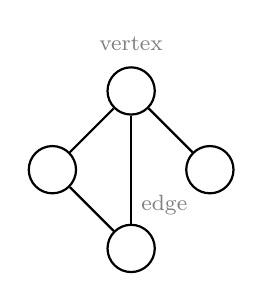
\begin{tikzpicture}
			\tikzset{
				basicnode/.style={
						shape=circle,
						draw=black,
						thick,
						fill=white,
						minimum size=6mm,
						inner sep=0pt
					}
			}

			\node[basicnode] (m1) at (0,0) {};
			\node[basicnode] (m2) at (-1,-1) {};
			\node[basicnode] (m3) at (1,-1) {};
			\node[basicnode] (m4) at (0,-2) {};

			\node[above of =m1, yshift=-4mm, smallgraytext] {vertex};

			\draw[thick] (m1) edge (m2);
			\draw[thick] (m1) edge (m3);
			\draw[thick] (m1) edge node[right, midway, yshift=-4.5mm, smallgraytext] {edge} (m4);
			\draw[thick] (m2) edge (m4);
		\end{tikzpicture}
	\end{figure}
\end{frame}

\begin{frame}
	\begin{defboxtop}
		A \highlight{\textbf{graph}} is a collection of vertices $V$ and edges, $E$, representing connections between pairs of vertices.

		\begin{figure}
			\centering
			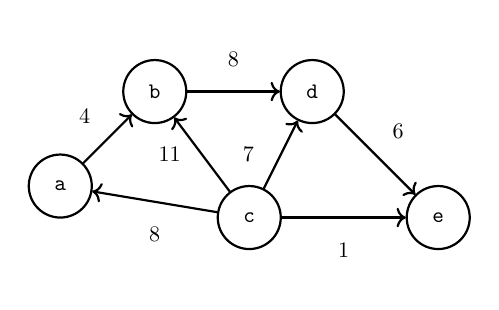
\begin{tikzpicture}[scale=0.8, transform shape]
				\node[defaultnode] (ta) at (0, 0.5) {\texttt{a}};
				\node[defaultnode] (tb) at (1.5, 2) {\texttt{b}};
				\node[defaultnode] (tc) at (3, 0) {\texttt{c}};
				\node[defaultnode] (td) at (4, 2) {\texttt{d}};
				\node[defaultnode] (te) at (6, 0) {\texttt{e}};

				\draw[defaultnode, ->] (ta) edge node[midway, above left] {$4$} (tb);
				\draw[defaultnode, <-] (ta) edge node[midway, below] {$8$} (tc);

				\draw[defaultnode, <-] (tb) edge node[midway, left] {$11$} (tc);
				\draw[defaultnode, ->] (tb) edge node[midway, above] {$8$} (td);

				\draw[defaultnode, ->] (tc) edge node[midway, left] {$7$} (td);
				\draw[defaultnode, ->] (tc) edge node[midway, below] {$1$} (te);

				\draw[defaultnode, ->] (td) edge node[midway, above right] {$6$} (te);
			\end{tikzpicture}
		\end{figure}
		\vspace{-8mm}
		\begin{center}
			\graytext{an example graph}
		\end{center}
	\end{defboxtop}
\end{frame}

\begin{frame}
	\begin{defboxside}
		Given a vertex, $v \in V$, we define:
		\begin{itemize}
			\item $\textsf{in}(v) \subseteq E$ as the set of \highlight{\textbf{in-coming}} edges
			\item $\textsf{out}(v) \subseteq E$ as the set of \highlight{\textbf{out-going}} edges
		\end{itemize}
		\begin{figure}
			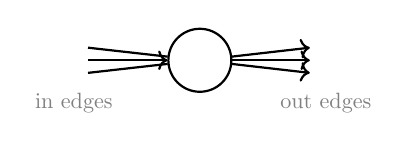
\begin{tikzpicture}[scale=0.8, transform shape]
				\node[opacity=0] at (-2,0) (l) {$u$};
				\node[defaultnode] at (0,0) (v) {};
				\node[opacity=0] at (2, 0) (r) {$w$};


				\node[below = 2mm of l] {\color{gray}{in edges}};
				\node[below = 2mm of r] {\color{gray}{out edges}};

				\draw[->, defaultnode] (v) -- (r);
				\draw[->, defaultnode] (v) -- (r.north west);
				\draw[->, defaultnode] (v) -- (r.south west);

				\draw[defaultnode] (l.north east) -- (v);
				\draw[->, defaultnode] (l) -- (v);
				\draw[defaultnode] (l.south east) -- (v);
			\end{tikzpicture}
		\end{figure}
	\end{defboxside}
\end{frame}

\begin{frame}
	\begin{defboxside}
		Given an edge, $e\in E$, we define:
		\begin{itemize}
			\item $\textsf{org}(e) \in V$ as the \highlight{\textbf{origin}}/\highlight{\textbf{parent}} vertex
			\item $\textsf{dst}(e) \in V$ as the \highlight{\textbf{destination}}/\highlight{\textbf{child}} vertex
			\item $\textsf{wgt}(e) \in \mathbb{R}$ as the \highlight{\textbf{weight}} of the edge (if it exists)
		\end{itemize}
		\begin{figure}
			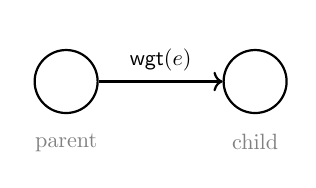
\begin{tikzpicture}[scale=0.8, transform shape]
				\node[defaultnode] at (0,0) (u) {};
				\node[below = 2mm of u] {\color{gray}{parent}};
				\node[defaultnode, circle, draw=black, inner sep=0] at (3, 0) (v) {};
				\node[below = 2mm of v] {\color{gray}{child}};
				\draw[->, defaultnode] (u) edge node[above=-2mm] {$\textsf{wgt}(e)$} (v);
			\end{tikzpicture}
		\end{figure}
		Two vertices, $u, v \in V$, are \highlight{\textbf{adjacent}} if they share at least one edge.
	\end{defboxside}
\end{frame}

\begin{frame}
	\begin{defboxbot}
		\item A \highlight{\textbf{path}} of length $k$ with origin vertex $u \in V$ and destination vertex $v \in V$ is a sequence of $k$ edges:\vspace{-1mm}
		\begin{center}
			$p = \big\langle e_0, e_1, e_2, \dots, e_{k} \big\rangle$
		\end{center}\vspace{-1mm}
		with $\textsf{org}(e_0) = \varnothing$, $\textsf{dst}(e_0) = u$, $\textsf{dst}(e_i) = \textsf{org}(e_{i+1})$, and $\textsf{dst}(e_k) = v$. \\[4mm]
		The total weight (or cost) of the path is $\textsf{cst}(p) = \sum_{e\in p}\textsf{wgt}(e)$.
		\begin{figure}
			\centering
			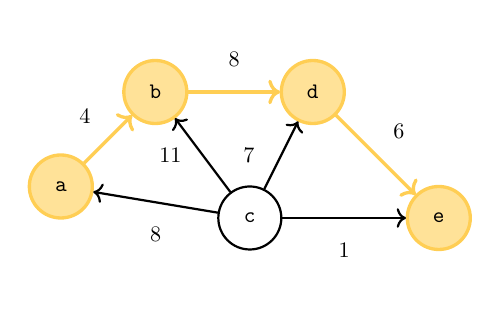
\begin{tikzpicture}[scale=0.8, transform shape]
				\node[newnode] (ta) at (0, 0.5) {\texttt{a}};
				\node[newnode] (tb) at (1.5, 2) {\texttt{b}};
				\node[defaultnode] (tc) at (3, 0) {\texttt{c}};
				\node[newnode] (td) at (4, 2) {\texttt{d}};
				\node[newnode] (te) at (6, 0) {\texttt{e}};

				\draw[newnode, ->] (ta) edge node[midway, above left] {$4$} (tb);
				\draw[defaultnode, <-] (ta) edge node[midway, below] {$8$} (tc);

				\draw[defaultnode, <-] (tb) edge node[midway, left] {$11$} (tc);
				\draw[newnode, ->] (tb) edge node[midway, above] {$8$} (td);

				\draw[defaultnode, ->] (tc) edge node[midway, left] {$7$} (td);
				\draw[defaultnode, ->] (tc) edge node[midway, below] {$1$} (te);

				\draw[newnode, ->] (td) edge node[midway, above right] {$6$} (te);
			\end{tikzpicture}
		\end{figure}
		\vspace{-8mm}
		\begin{center}
			\graytext{an example path on a graph}
		\end{center}
	\end{defboxbot}
\end{frame}

\begin{frame}
	\begin{thmbox}
		A graph is called \highlight{\textbf{simple}} iff there is at most one edge from any vertex to any vertex.
		\begin{figure}
			\centering
			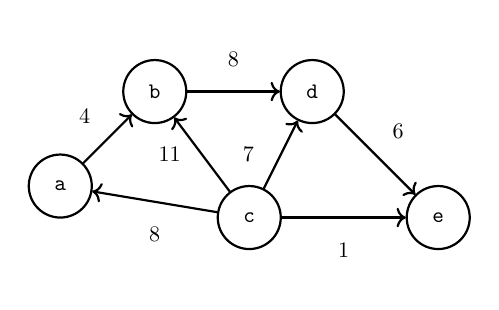
\begin{tikzpicture}[scale=0.8, transform shape]

				\node[defaultnode] (ta) at (0, 0.5) {\texttt{a}};
				\node[defaultnode] (tb) at (1.5, 2) {\texttt{b}};
				\node[defaultnode] (tc) at (3, 0) {\texttt{c}};
				\node[defaultnode] (td) at (4, 2) {\texttt{d}};
				\node[defaultnode] (te) at (6, 0) {\texttt{e}};

				\draw[defaultnode, ->] (ta) edge node[midway, above left] {$4$} (tb);
				\draw[defaultnode, <-] (ta) edge node[midway, below] {$8$} (tc);

				\draw[defaultnode, <-] (tb) edge node[midway, left] {$11$} (tc);
				\draw[defaultnode, ->] (tb) edge node[midway, above] {$8$} (td);

				\draw[defaultnode, ->] (tc) edge node[midway, left] {$7$} (td);
				\draw[defaultnode, ->] (tc) edge node[midway, below] {$1$} (te);

				\draw[defaultnode, ->] (td) edge node[midway, above right] {$6$} (te);
			\end{tikzpicture}
		\end{figure}
		\vspace{-8mm}
		\begin{center}
			\graytext{an example graph}
		\end{center}
		In such graphs, we represent an edge $e \in E$ as $\left(\textsf{org}(e), \textsf{dst}(e)\right)$.
	\end{thmbox}

\end{frame}

\begin{frame}
	\begin{figure}
		\centering
		\begin{tikzpicture}[scale=0.8, transform shape]
			\draw[opacity=0] (-1.5,-2) rectangle (11,4);

			\labeledimgnodetikz[defaultnode]{\footnotesize\texttt{A}}{1.5}{2}{tA}{images/radio_tower.png}{0.044};
			\labeledimgnodetikz[defaultnode]{\footnotesize\texttt{B}}{3}{0}{tB}{images/radio_tower.png}{0.044};
			\labeledimgnodetikz[defaultnode]{\footnotesize\texttt{C}}{4}{2}{tC}{images/radio_tower.png}{0.044};
			\labeledimgnodetikz[defaultnode]{\footnotesize\texttt{D}}{6}{0.5}{tD}{images/radio_tower.png}{0.044};
			\labeledimgnodetikz[defaultnode]{\footnotesize\texttt{E}}{8}{2}{tE}{images/radio_tower.png}{0.044};

			\imgnodetikz[defaultnode]{empty}{0}{0.5}{server}{images/server.png}{0.052};
			\imgnodetikz[defaultnode]{empty}{6.5}{3}{phone}{images/phone.png}{0.052};
			\imgnodetikz[defaultnode]{empty}{7.5}{-1}{computer}{images/computer.png}{0.052};
			\imgnodetikz[defaultnode]{empty}{9.5}{0.5}{router}{images/router.png}{0.052};


			\draw[defaultnode] (server) edge node[midway, above left] {$4$} (tA);
			\draw[defaultnode] (server) edge node[midway, below] {$8$} (tB);

			\draw[defaultnode] (tA) edge node[midway, left] {$11$} (tB);
			\draw[defaultnode] (tA) edge node[midway, above] {$8$} (tC);

			\draw[defaultnode] (tB) edge node[midway, left] {$7$} (tC);
			\draw[defaultnode] (tB) edge node[midway, below] {$1$} (tD);

			\draw[defaultnode] (tC) edge node[midway, above] {$2$} (phone);
			\draw[defaultnode] (tC) edge node[midway, above right] {$6$} (tD);

			\draw[defaultnode] (tD) edge node[midway, below left] {$2$} (computer);

			\draw[defaultnode] (phone) edge node[midway, above] {$7$} (tE);
			\draw[defaultnode] (phone) edge node[midway, right] {$4$} (computer);

			\draw[defaultnode] (tE) edge node[midway, right] {$14$} (computer);
			\draw[defaultnode] (tE) edge node[midway, above right] {$9$} (router);

			\draw[defaultnode] (computer) edge node[midway, below right] {$10$} (router);
		\end{tikzpicture}
	\end{figure}
	\begin{center}
		\graytext{
			a graph representing the devices in a network; each vertex
			\tikz[baseline=-0.6ex]{\node[defaultnode, scale=0.3] {}; }
			represents a device,\\ and an edge
			\tikz[baseline=-0.5ex]{\draw[thick] (0,0) -- (0.5,0);}
			is placed between pairs of devices that are nearby
		}
	\end{center}
\end{frame}

\begin{frame}[fragile]
	A \texttt{Graph} stores \texttt{Vertex} and \texttt{Edge} objects and supports the following operations:\\~\\
	\begin{itemize}
		\item \highlight{\texttt{get\_vertex}} \\
		      \graytext{returns a vertex (if it exists)}\\[-1mm]
		      \begin{lstlisting}[style=mypython]
get_vertex(key: Key) -> Optional[Vertex]
\end{lstlisting}

		\item \highlight{\texttt{get\_vertices}} \\
		      \graytext{returns all vertices}\\[-1mm]
		      \begin{lstlisting}[style=mypython]
get_vertices() -> List[Vertex]
\end{lstlisting}
	\end{itemize}

\end{frame}

\begin{frame}[fragile]
	\begin{itemize}
		\item \highlight{\texttt{get\_edges\_btw}} \\
		      \graytext{returns all edges from one vertex to another}\\[-1mm]
		      \begin{lstlisting}[style=mypython]
get_edges_btw(key1: Key, key2: Key) -> List[Edge]
\end{lstlisting}

		\item \highlight{\texttt{get\_edges\_from}} \\
		      \graytext{returns all edges from a vertex (if it exists)}\\[-1mm]
		      \begin{lstlisting}[style=mypython]
get_edges_from(key: Key) -> List[Edge]
\end{lstlisting}

		\item \highlight{\texttt{get\_edges\_to}} \\
		      \graytext{returns all edges to a vertex (if it exists)}\\[-1mm]
		      \begin{lstlisting}[style=mypython]
get_edges_to(key: Key) -> List[Edge]
\end{lstlisting}

		\item \highlight{\texttt{get\_edges}} \\
		      \graytext{returns all edges between any two vertices}\\[-1mm]
		      \begin{lstlisting}[style=mypython]
get_edges() -> List[Edge]
\end{lstlisting}

	\end{itemize}
\end{frame}

\begin{frame}[fragile]

	\begin{itemize}

		\item \highlight{\texttt{insert\_vertex}} \\
		      \graytext{adds a vertex}\\[-1mm]
		      \begin{lstlisting}[style=mypython]
insert_vertex(key: Key, obj: Object) -> Optional[Vertex]
\end{lstlisting}

		\item \highlight{\texttt{insert\_edge}} \\
		      \graytext{adds/updates an edge from one vertex to another}\\[-1mm]
		      \begin{lstlisting}[style=mypython]
insert_edge(key1: Key, key2: Key, wgt: Integer) -> Optional[Edge]
\end{lstlisting}

	\end{itemize}
\end{frame}

\begin{frame}{Graphs (via Adjacency Lists)}
	\begin{center}
		\Large \highlight{\texttt{Graph}} \\[1mm]
		\normalsize\color{gray} (via Adjacency Lists)
	\end{center}
\end{frame}

\begin{frame}[fragile]
	\begin{thmboxtop}
		\highlight{\texttt{Graph}} \\
		\graytext{(via Adjacency Lists)}
		\begin{lstlisting}[style=mypython]
class Vertex:
# attributes    
    # the key of this vertex
    key: Key
    
    # list of all incoming edges
    in_edges: List[Edge]

    # list of all outgoing edges
    out_edges: List[Edge]

    # the object of this vertex
    obj: Object
\end{lstlisting}
	\end{thmboxtop}
\end{frame}

\begin{frame}[fragile]
	\begin{thmboxside}
		\begin{lstlisting}[style=mypython, firstnumber=last]
class Edge:
# attributes    
    # the origin of this edge
    from: Vertex
    
    # the destination of this edge
    to: Vertex
    
    # the weight of this edge
    wgt: Integer
\end{lstlisting}
	\end{thmboxside}
\end{frame}

\begin{frame}[fragile]
	\begin{thmboxbot}
		\begin{lstlisting}[style=mypython, firstnumber=last]
class Graph:
# attributes
    # the vertices
    vertices: Dict[Key, Vertex]

    # the edges
    edges: List[Edge]

# functions
    ...
\end{lstlisting}
	\end{thmboxbot}
\end{frame}

\begin{frame}[fragile]
	\begin{proofbox}
		\begin{lstlisting}[style=mypython]
def get_vertex(self: Graph, key: Key) -> Optional[Vertex]:
    return self.vertices.get(key)
\end{lstlisting}
	\end{proofbox}
\end{frame}

\begin{frame}[fragile]
	\begin{proofbox}
		\begin{lstlisting}[style=mypython]
def get_vertices(self: Graph) -> List[Vertex]:
    return self.vertices.get_objs()
\end{lstlisting}
	\end{proofbox}
\end{frame}

\begin{frame}[fragile]
	\begin{proofbox}
		\begin{lstlisting}[style=mypython]
def get_edges_btw(self: Graph, key1: Key, key2: Key) -> List[Edge]:
    edges = List[Edge]()
    for edge in self.vertices.get(key1).out_edges:
        if edge.to.key is key2:
            edges.append(edge)
    return edges
\end{lstlisting}
	\end{proofbox}
\end{frame}

\begin{frame}[fragile]
	\begin{proofbox}
		\begin{lstlisting}[style=mypython]
def get_edges_from(self: Graph, key: Key) -> List[Edge]:
    return self.vertices.get(key).out_edges    
\end{lstlisting}
	\end{proofbox}
\end{frame}

\begin{frame}[fragile]
	\begin{proofbox}
		\begin{lstlisting}[style=mypython]
def get_edges_to(self: Graph, key: Key) -> List[Edge]:
    return self.vertices.get(key).in_edges  
\end{lstlisting}
	\end{proofbox}
\end{frame}

\begin{frame}[fragile]
	\begin{proofbox}
		\begin{lstlisting}[style=mypython]
def get_edges(self: Graph) -> List[Edge]:
   return self.edges
\end{lstlisting}
	\end{proofbox}
\end{frame}


\begin{frame}
	\begin{table}
		\begin{tabular}{@{} r | l @{} }
			\highlight{\textbf{Property}}                      &                                    \\[1mm]\hline
			\multirow{1}{*}{Time Complexity}                   &                                    \\
			\color{gray}\footnotesize\texttt{get\_vertex}      & \color{gray}\footnotesize $O(1)$   \\[1mm]
			\color{gray}\footnotesize\texttt{get\_vertices}    & \color{gray}\footnotesize $O(|V|)$ \\[1mm]
			\color{gray}\footnotesize\texttt{get\_edges\_btw}  & \color{gray}\footnotesize $O(|V|)$ \\[1mm]
			\color{gray}\footnotesize\texttt{get\_edges\_from} & \color{gray}\footnotesize $O(1)$   \\[1mm]
			\color{gray}\footnotesize\texttt{get\_edges\_to}   & \color{gray}\footnotesize $O(1)$   \\[1mm]
			\color{gray}\footnotesize\texttt{get\_edges}       & \color{gray}\footnotesize $O(1)$   \\[1mm]
			Space Complexity                                   & $O(|V|+|E|)$
		\end{tabular}
	\end{table}
	\begin{center}
		\graytext{properties of the \texttt{Graph} data-structure (via Adjacency Lists)}
	\end{center}
	\renewcommand\thefootnote{}\footnotetext{\color{gray} Assumptions: $V =$ \texttt{Graph.vertices.size}, $E =$ \texttt{Graph.edges.size}}
\end{frame}

\begin{frame}{Graphs (via Adjacency Matrices)}
	\begin{center}
		\Large \highlight{\texttt{Graph}} \\[1mm]
		\normalsize\color{gray} (via Adjacency Matrices)
	\end{center}
\end{frame}

\begin{frame}[fragile]
	\begin{thmboxtop}
		\highlight{\texttt{Graph}} \\
		\graytext{(via Adjacency Matrices)}
		\begin{lstlisting}[style=mypython]
class Vertex:
# attributes
    # the key of this vertex
    key: Key

    # the object of this vertex
    obj: Object
\end{lstlisting}
	\end{thmboxtop}
\end{frame}

\begin{frame}[fragile]
	\begin{thmboxside}
		\begin{lstlisting}[style=mypython, firstnumber=last]
class Edge:
# attributes
    # the origin of this edge
    from: Vertex

    # the destination of this edge
    to: Vertex
    
    # the weight of this edge
    wgt: Integer
\end{lstlisting}
	\end{thmboxside}
\end{frame}

\begin{frame}[fragile]
	\begin{thmboxbot}
		\begin{lstlisting}[style=mypython, firstnumber=last]
class Graph:
# attributes
     # the vertices
    vertices: Dict[Key, Vertex]
    
    # the edges
    edges: Dict[Key, Dict[Key, Optional[Edge]]]

# functions
    ...
\end{lstlisting}
	\end{thmboxbot}
\end{frame}

\begin{frame}[fragile]
	\begin{proofbox}
		\begin{lstlisting}[style=mypython]
def get_vertex(self: Graph, key: Key) -> Optional[Vertex]:
    return self.vertices.get(key)
\end{lstlisting}
	\end{proofbox}
\end{frame}

\begin{frame}[fragile]
	\begin{proofbox}
		\begin{lstlisting}[style=mypython]
def get_vertices(self: Graph) -> List[Vertex]:
    return self.vertices.get_objs()
\end{lstlisting}
	\end{proofbox}
\end{frame}

\begin{frame}[fragile]
	\begin{proofbox}
		\begin{lstlisting}[style=mypython]
def get_edges_btw(self: Graph, key1: Optional[Key], key2: Optional[Key]) -> List[Edge]:
    edges = List[Edge]()
    edge = self.edges[key1][key2]
    if edge is not None:
        edges.append(edge)
    return edges
\end{lstlisting}
	\end{proofbox}
\end{frame}

\begin{frame}[fragile]
	\begin{proofbox}
		\begin{lstlisting}[style=mypython]
def get_edges_from(self: Graph, key: Key) -> List[Edge]:
    return self.edges[key].get_objs()
\end{lstlisting}
	\end{proofbox}
\end{frame}

\begin{frame}[fragile]
	\begin{proofbox}
		\begin{lstlisting}[style=mypython]
def get_edges_to(self: Graph, key: Key) -> List[Edge]:
    edges = List[Edge]()
    for key_from in self.edges.get_keys():
        for edge in self.edges[key_from].get_objs():
            if edge is not None and edge.to.key is key:
                edges.append(edge)    
    return edges
\end{lstlisting}
	\end{proofbox}
\end{frame}

\begin{frame}[fragile]
	\begin{proofbox}
		\begin{lstlisting}[style=mypython]
def get_edges(self: Graph) -> List[Edge]:
    edges = List[Edge]()
    for key_from in self.edges.get_keys():
        for edge in self.edges[key_from].get_objs():
            if edge is not None:
                edges.append(edge)    
    return edges
\end{lstlisting}
	\end{proofbox}
\end{frame}

\begin{frame}
	\begin{table}
		\begin{tabular}{@{} r | l @{} }
			\highlight{\textbf{Property}}        &                       \\[1mm]\hline
			\multirow{1}{*}{Time Complexity}     &                       \\
			\graytext{\texttt{get\_vertex}}      & \graytext{$O(1)$}     \\[1mm]
			\graytext{\texttt{get\_vertices}}    & \graytext{$O(|V|)$}   \\[1mm]
			\graytext{\texttt{get\_edges\_btw}}  & \graytext{$O(1)$}     \\[1mm]
			\graytext{\texttt{get\_edges\_from}} & \graytext{$O(|V|)$}   \\[1mm]
			\graytext{\texttt{get\_edges\_to}}   & \graytext{$O(|V|^2)$} \\[1mm]
			\graytext{\texttt{get\_edge}}        & \graytext{$O(|V|^2)$} \\[1mm]
			Space Complexity                     & $O(|V|^2)$
		\end{tabular}
	\end{table}
	\begin{center}
		\graytext{properties of the \texttt{Graph} data-structure (via Adjacency Matrices)}
	\end{center}
	\renewcommand\thefootnote{}\footnotetext{\color{gray} Assumptions: $V =$ \texttt{Graph.vertices.size}, $E =$ \texttt{Graph.matrix.size}}
\end{frame}


\end{document}